\documentclass{article}

\usepackage[preprint]{neurips_2026}

\usepackage[utf8]{inputenc}
\usepackage[T1]{fontenc}
\usepackage{hyperref}
\usepackage{url}
\usepackage{booktabs}
\usepackage{amsfonts}
\usepackage{amsmath}
\usepackage{amssymb}
\usepackage{mathtools}
\usepackage{amsthm}
\usepackage{nicefrac}
\usepackage{microtype}
\usepackage{xcolor}
\usepackage{graphicx}
\usepackage{subcaption}
\usepackage[capitalize,noabbrev]{cleveref}

\theoremstyle{plain}
\newtheorem{theorem}{Theorem}[section]
\newtheorem{proposition}[theorem]{Proposition}
\newtheorem{lemma}[theorem]{Lemma}
\theoremstyle{definition}
\newtheorem{definition}[theorem]{Definition}

\newcommand{\subrparagraph}[1]{\vspace{1mm}\noindent\textbf{#1}}
\newcommand{\subsparagraph}[1]{\vspace{0.0mm}\noindent\textbf{#1}}
\newcommand{\rparagraph}[1]{\vspace{1.2mm}\noindent\textbf{#1.}}
\newcommand{\rparagraphnodot}[1]{\vspace{1.2mm}\noindent\textbf{#1}}
\newcommand{\sparagraph}[1]{\vspace{0.0mm}\noindent\textbf{#1.}}

\newcommand{\ours}{{\textsc{Scrl}}}
\newcommand{\oursfull}{RL-Guided Skill Creator}%

\definecolor{Gray}{gray}{0.92}

\definecolor{ourred}{HTML}{E65100}
\definecolor{ourblue}{HTML}{1565C0}

\definecolor{paleblue}{HTML}{7EA6E0}
\definecolor{palered}{HTML}{F19C99}
\definecolor{palegreen}{HTML}{A8D5A2}

\definecolor{plotred}{HTML}{f77189}
\definecolor{plotgreen}{HTML}{33b07a}
\definecolor{plotpurple}{HTML}{cc7af4}

\definecolor{stage1}{HTML}{34A853}
\definecolor{stage2}{HTML}{A680B8}
\definecolor{stage3}{HTML}{009999}

\definecolor{mainboxbg}{HTML}{F7F9FC}
\definecolor{mainboxborder}{HTML}{A1C6EA}

\definecolor{g-red}{RGB}{213, 66, 56}
\definecolor{g-green}{RGB}{49, 149, 79}

\usepackage{colortbl}
\usepackage{float}
\usepackage{multirow}
\usepackage{algorithm}
\usepackage{algorithmic}
\usepackage{enumitem}


\title{\ours: RL-Guided Skill Creator\\for Agentic Skill-Policy Co-Evolution}

\author{%
  Anonymous Authors
}

\begin{document}

\maketitle

\begin{abstract}
% TODO: Abstract to be written.
\end{abstract}

%=============================================================================
\section{Introduction}
%=============================================================================

Large language models (LLMs) \citep{brown2020language, chung2024scaling} have enabled autonomous agents capable of reasoning, tool use, and multi-turn interaction with complex environments \citep{yao2023react, jimenez2023swe, su2025learnbyinteract}. Reinforcement learning (RL) with verifiable rewards (RLVR) has further advanced these capabilities, enabling agents to discover effective policies through direct environment interaction \citep{shao2024deepseekmath, guo2025deepseek, jin2025search, xue2025simpletir}.

While RL provides a powerful learning signal, each training step is expensive: every GRPO step generates $G$ multi-turn rollouts per question, each involving multiple rounds of model inference and environment interaction. This computational cost motivates maximizing the utility of each rollout, extracting not only policy gradients but also insights about what strategies succeed and fail.

A promising direction for improving agent efficiency is \textit{skills}: modular, reusable behavioral patterns that guide agent actions in specific situations. Anthropic's Skill Creator \citep{anthropic2025skillcreator} pioneered the automated creation of such modular skills from agent experience, demonstrating that structured skill libraries can dramatically improve agent capabilities. SkillRL \citep{xia2025skillrl} distills teacher-model knowledge into skill banks that augment RL training. Other approaches accumulate experiential knowledge through verbal reinforcement \citep{shinn2023reflexion} or episodic learning \citep{zhao2024expel}. However, these approaches treat skills as \textit{static} artifacts, created before or outside the RL training loop and then frozen during policy optimization.

The fundamental limitation of static skills mirrors that of static instructions in RLVR \citep{zhou2025inspo}: the optimal skill set is not known \textit{a priori} and changes as the agent's policy improves. A skill that scaffolds a weak policy (e.g., ``always search before answering'') may constrain a stronger policy that has internalized this behavior. Conversely, a skill addressing subtle failure modes only becomes relevant after the policy has mastered basic competencies. Static skill banks, whether distilled from teacher models \citep{xia2025skillrl} or accumulated from fixed experience \citep{zhao2024expel, shinn2023reflexion}, cannot adapt to these shifting needs and risk either under-guiding or over-constraining the evolving policy \citep{soylu-etal-2024-fine, liu2025understanding}. This creates a core tension: \emph{skills guide what can be instructed; policy learns what must be discovered}.

To bridge this gap, we propose \ours, an \textbf{RL}-guided \textbf{S}kill \textbf{C}reator for agentic skill-policy co-evolution. \ours~integrates skill creation and evolution as dynamic components of the RL loop, delivering two major innovations. First, we introduce an \textit{assertion-driven skill creator pipeline} that creates modular, trigger-based skills from failed trajectories. A rule-based assertion grader provides structured failure diagnosis with quantitative prevalence statistics, an LLM-based analyzer evolves the diagnostic criteria and identifies representative failures, and an LLM-based optimizer proposes targeted skill modules, each paired with a \textit{trigger condition} that determines when it activates at the action level during rollouts. This enables situational guidance without prompt bloat. Second, we propose an \textit{RL-guided skill evolution mechanism via Thompson Sampling} \citep{thompson1933likelihood}, where GRPO rollouts serve \textbf{triple duty}: policy optimization via standard gradients, failure collection for skill creation via a bounded reservoir, and bandit evaluation for skill evolution via per-skill Thompson Sampling. Each proposed skill is tested as a bandit decision by stochastically including or excluding it in episodes where its trigger fires, with Beta-Binomial posteriors providing principled, sample-efficient accept/reject decisions. Zero additional rollouts are required beyond standard GRPO training.

We validate \ours~through extensive experiments on three diverse agentic benchmarks, WebShop \citep{yao2022webshop}, multi-hop question answering with search tools, and ALFWorld \citep{shridharalfworld}, across three model scales (4B, 8B, 14B parameters). \ours~achieves substantial convergence speedup over GRPO and static skill baselines, with ablation studies confirming the contribution of each component. The entire skill creation and evolution process incurs only marginal computational overhead: a few LLM calls per evolution cycle, with no additional rollouts.


%=============================================================================
\section{Preliminaries}
%=============================================================================

\subsection{Reinforcement Learning with Tool-Using}
We formalize multi-turn tool-using as a Markov Decision Process (MDP) \citep{hauskrecht2013hierarchical}, where the LLM-based agent, governed by its policy $\pi$ and parameterized by the weights $\theta$, interacts with an external environment by calling a tool engine $\mathcal{T}$. It generates a trajectory $\tau$ as its state that comprises multiple turns of interactions: $\tau=(q, \mathcal{S}_{\text{active}}, a_{0},o_{0},\dots,a_{k-1},o_{k-1},a_{k})$, where $q$ is the task input and $\mathcal{S}_{\text{active}} \subseteq \mathcal{S}$ denotes the set of active skills injected into the prompt. $a_k$ is the response from the LLM given the history trajectory up to turn $k$, such that $a \sim \pi_{\theta}(\cdot | q, \mathcal{S}_{\text{active}};\mathcal{T})$. The observation $o$ is the feedback from the environment by calling the tool engine, $o_k=\mathcal{T}(a_k)$, which is concatenated in an interleaved manner with the action.

The learning objective of RL is to optimize the policy parameters $\theta$ by maximizing the expected returns over a distribution of tasks $\mathcal{D}$, where $r(\tau)$ defines the reward function. In RLVR, the reward is typically defined via a rule-based verifier, such as an exact match or task-completion reward $r(\tau)\in\{0, 1\}$. The learning objective is:
\begin{equation}
    \max_{\pi_\theta} \mathbb{E}_{q \sim \mathcal{D},\, \tau \sim \pi_\theta(\cdot|q, \mathcal{S}_{\text{active}};\mathcal{T})} \left[ r(\tau)
    \right].
    \label{eq:rl_objective}
\end{equation}

\subsection{Group Relative Policy Optimization (GRPO)}
Group Relative Policy Optimization (GRPO) \citep{shao2024deepseekmath} is a policy optimization method that derives from Proximal Policy Optimization (PPO) \citep{schulman2017proximal} and obviates the need for a separate value function, instead using group-wise sampling to estimate the advantage function $\hat{A}$ based on relative performance within a group $G$. For each task $q\sim\mathcal{D}$, GRPO samples a group of trajectories $\{\tau_i\}_{i=1}^G$ from the old policy $\pi_{\theta_{\text{old}}}(\cdot \mid q, \mathcal{S}_{\text{active}}; \mathcal{T})$ and optimizes:
\begin{equation}
\begin{aligned}
&\mathcal{J}_{\text{GRPO}}(\theta) = \mathbb{E}_{\tau \sim \pi_{\text{old}}} \Bigg[ \frac{1}{G} \sum_{i=1}^G \frac{1}{\sum_t \mathcal{I}_{i,t}} \sum_{t=1}^{|\tau_i|}\mathcal{I}_{i,t} \cdot \min \left( \rho_{i,t}\hat{A}_{i}, \text{clip}(\rho_{i,t}, 1{-}\epsilon, 1{+}\epsilon) \hat{A}_{i} \right)  - \beta \mathbb{D}_{\text{KL}} \Bigg],
\end{aligned}
\label{eq:grpo}
\end{equation}
where $\rho_{i,t}(\theta) = {\pi_\theta(\tau_{i,t}|\tau_{i,<t})}/{\pi_{\theta_{\text{old}}}(\tau_{i,t}|\tau_{i,<t})}$ is the token-level importance ratio, $\hat{A}_i = ({r_i - \text{mean}(\{r_j\}_{j=1}^{G})})/{\text{std}(\{r_j\}_{j=1}^{G})}$ is the group-normalized advantage, $\epsilon$ is the clip ratio, and $\beta$ controls the KL divergence penalty $\mathbb{D}_{\text{KL}}(\pi_\theta \| \pi_{\text{ref}})$ with respect to the reference policy. The indicator function $\mathcal{I}_{i,t}$ masks out observation tokens $o$ so that policy gradients are computed only over the agent's own action tokens $a$ \citep{jin2025search, xue2025simpletir}.


%=============================================================================
\section{RL-Guided Skill Creation (\ours)}
\label{sec:method}
%=============================================================================

The conventional RLVR approach treats any auxiliary guidance, whether instructions \citep{zhou2025inspo} or skills \citep{xia2025skillrl}, as a static, pre-defined input. This constrains the agent's exploration and may result in suboptimal convergence, as the ideal guidance changes with the evolving policy. \ours~re-frames skill design as a \textit{dynamic} and \textit{integral} component of the RL loop, enabling skills and policy to co-evolve in an online setting. The core of \ours~is composed of two synergistic components: an assertion-driven pipeline that creates modular skills from failure analysis (\S\ref{sec:skill_creator}), and an RL-guided evolution mechanism that tests and prunes skills via Thompson Sampling within GRPO rollouts (\S\ref{sec:skill_evolution}).

\begin{figure*}[!t]
\centering
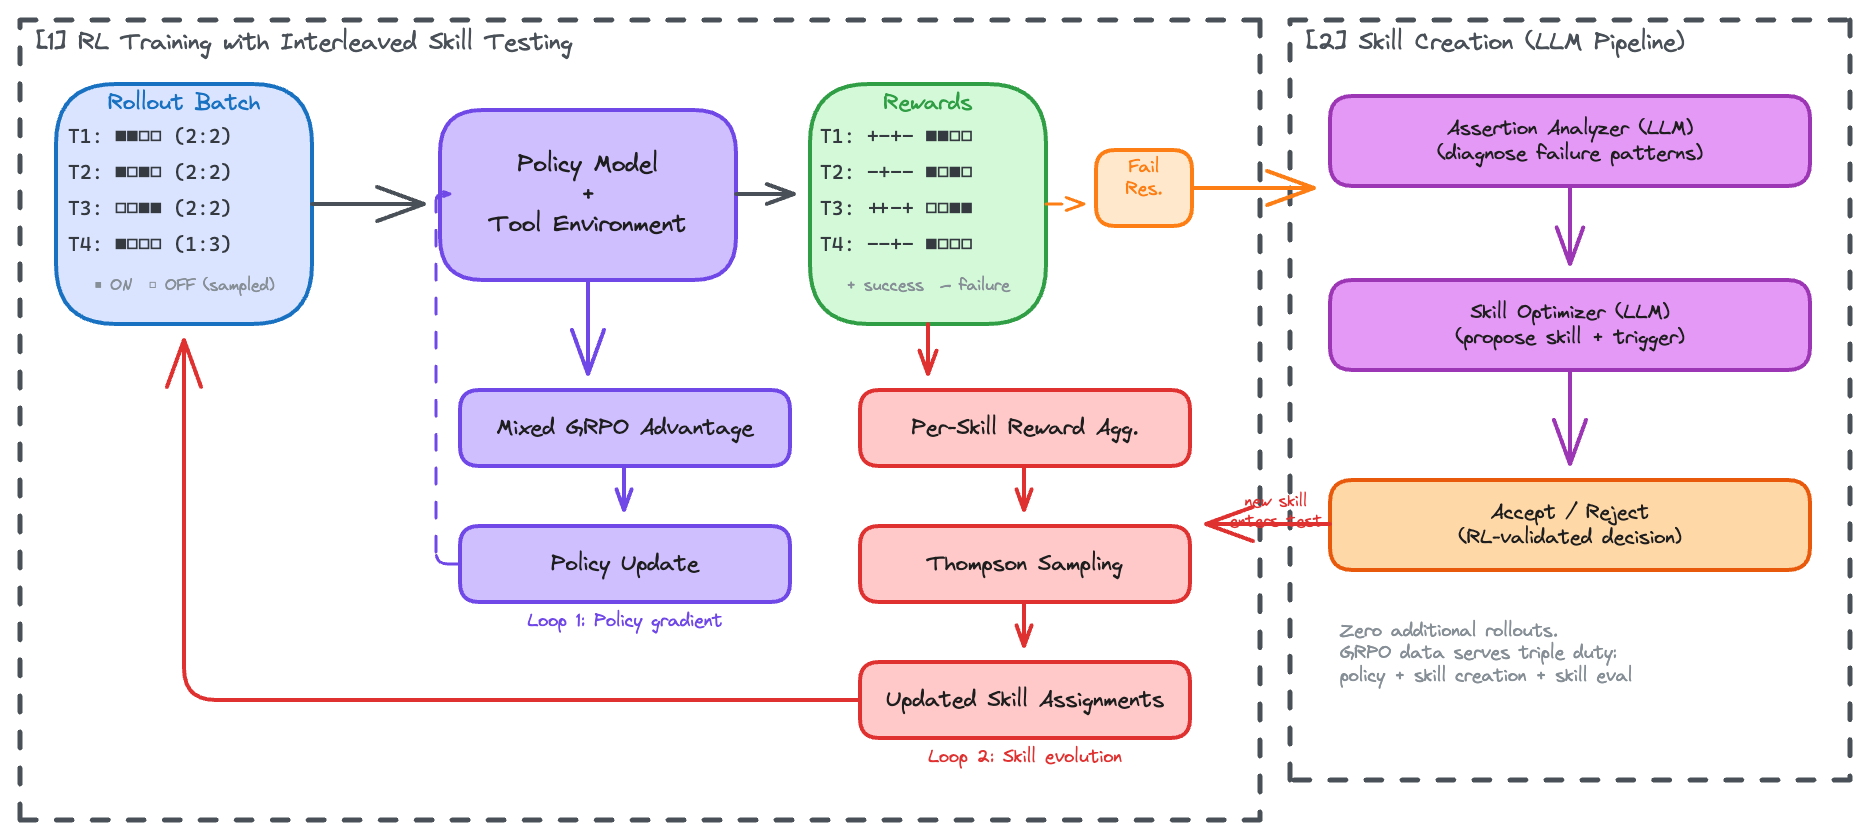
\includegraphics[width=\textwidth]{figures/diagram.png}
\caption{The \ours~pipeline. \textbf{Left}: Policy optimization with interleaved skill testing via Thompson Sampling. Each proposed skill is stochastically included or excluded at the trigger point, and the RL reward signal determines whether the skill is accepted or pruned. \textbf{Right}: Skill creation from failure trajectories. An assertion grader diagnoses failures quantitatively, an LLM-based analyzer identifies patterns, and a skill optimizer proposes modular, trigger-based skills.}
\label{fig:pipeline}
\end{figure*}

\subsection{Assertion-Driven Skill Creator Pipeline}
\label{sec:skill_creator}

We first define the \textit{skill module} as the atomic unit of guidance in \ours. A skill $S_k = (c_k, \text{trig}_k)$ consists of content $c_k$ (a structured instruction snippet) and a trigger condition $\text{trig}_k$ that determines when the skill activates during a rollout. Trigger conditions are parameterized by type and pattern, allowing the skill optimizer to choose from several activation modes (e.g., every step, only at the beginning, or only when a specific action pattern is observed). The skill bank $\mathcal{S} = \{S_1, \ldots, S_K\}$ collects all active skills. Skills are \textit{modular}: each targets a specific failure mode and activates only when its trigger condition is met, enabling compositional guidance without prompt bloat.

The skill creator pipeline adapts the Skill Creator paradigm, originally designed for human-in-the-loop development, for automated use within RL training. The input is failed GRPO rollouts collected over time into a bounded failure reservoir $\mathcal{R}$. The pipeline operates in three stages, triggered periodically (every $K_e$ GRPO steps) when the system is not already testing a candidate skill.

\rparagraph{Assertion Grading and Analysis}
The assertion grader $\mathcal{G}$ maintains a dynamic set of rule-based assertions $\mathcal{A} = \{a_j\}_{j=1}^M$, where each assertion $a_j = (\text{check}_j, \text{params}_j)$ is a predicate over trajectories (e.g., \texttt{action\_exists}, \texttt{action\_before}, \texttt{final\_action}). Given the failure reservoir $\mathcal{R}$, the grader evaluates every trajectory against all assertions, producing per-assertion pass rates $p_j = |\mathcal{R}|^{-1} \sum_{\tau \in \mathcal{R}} \mathbf{1}[\text{check}_j(\tau, \text{params}_j)]$ that quantify the prevalence of specific behavioral patterns. The grader is entirely rule-based with no LLM calls.

An LLM-based assertion analyzer $\mathcal{Z}$ then receives the pass rates, a stratified sample of trajectories from $\mathcal{R}$, and a summary of the current skill bank $\mathcal{S}$. The analyzer \textit{evolves the assertion set} $\mathcal{A}$ via operations (add, delete, modify), adapting the diagnostic criteria to the current policy's failure landscape. It also produces a \textit{failure diagnosis} $\mathcal{F}_{\text{diag}}$ with prevalence-ranked patterns and selects representative episodes $\mathcal{E}_{\text{sel}}$ for the skill optimizer.

\rparagraph{Skill Optimization}
An LLM-based skill optimizer $\mathcal{O}$ receives the failure diagnosis $\mathcal{F}_{\text{diag}}$, the selected episodes $\mathcal{E}_{\text{sel}}$, a summary of the current skill bank, and action-pattern frequency statistics from recent rollouts. It proposes exactly \textit{one} new skill module $S_{\text{new}} = (c_{\text{new}}, \text{trig}_{\text{new}})$. Before entering Thompson Sampling evaluation, the proposed skill must pass a \textit{trigger rate gate}: we estimate the fraction of reservoir episodes where the trigger would fire, and require $\hat{p}_{\text{trigger}} \geq \delta$ (default $\delta = 0.1$). If the gate fails, the optimizer is re-called with feedback about the rejection reason, up to 3 retries. This ensures proposed skills are testable within a reasonable number of episodes.


\subsection{RL-Guided Skill Evolution with Thompson Sampling}
\label{sec:skill_evolution}

Rather than relying on a human judge or external validation, \ours~uses the RL training signal itself to evolve skills. Inspired by instruction-policy co-evolution \citep{zhou2025inspo}, the evolution mechanism integrates skill evaluation directly into GRPO rollouts through trigger-based injection and Thompson Sampling \citep{thompson1933likelihood, russo2018tutorial}.

\rparagraph{Trigger-Based Skill Injection}
At each step $t$ of a multi-turn episode, the trigger matcher determines which skills are injected into the prompt. Each skill's trigger condition $\text{trig}_k$ is a predicate over the current step index and the previous action, allowing the skill optimizer to specify diverse activation patterns:
\begin{equation}
    \mathcal{S}_{\text{active}}^{(t)} = \{S_k \in \mathcal{S} : \text{trig}_k(t, a_{t-1}) = 1 \wedge \text{status}(S_k) \neq \text{excluded}\},
    \label{eq:trigger}
\end{equation}
where the status of skills under test is determined by the Thompson Sampling mechanism described below. This per-step trigger mechanism allows different skills to activate at different moments within a single episode, providing targeted guidance without inflating every prompt. The specific trigger types and their semantics are detailed in Appendix~\ref{app:triggers}.

\rparagraph{Thompson Sampling for Skill Evaluation}
When a new skill $S_{\text{new}}$ is proposed by the creator pipeline, it enters a \textit{bandit evaluation} phase embedded within GRPO rollouts. The key question is whether including this skill improves episode outcomes. We frame this as a two-armed bandit problem: the \textit{include} arm injects the skill when its trigger fires, and the \textit{exclude} arm withholds it. Each arm maintains a Beta-Binomial posterior:
\begin{equation}
    \theta_{\text{inc}} \sim \text{Beta}(\alpha_{\text{inc}}, \beta_{\text{inc}}), \quad \theta_{\text{exc}} \sim \text{Beta}(\alpha_{\text{exc}}, \beta_{\text{exc}}),
    \label{eq:thompson_posteriors}
\end{equation}
initialized with uniform priors $\text{Beta}(1, 1)$. At the start of each episode, the include/exclude decision is sampled via Thompson Sampling (Use 7, it's approximated):
\begin{equation}
    d = \mathbf{1}[\theta_{\text{inc}} > \theta_{\text{exc}}], \quad \text{with } \Pr(\text{include}) = \text{clamp}\!\left(\Pr(\theta_{\text{inc}} > \theta_{\text{exc}}),\, p_{\min},\, p_{\max}\right),
    \label{eq:thompson_decision}
\end{equation}
where $p_{\min} = 0.15$ and $p_{\max} = 0.85$ ensure both arms are always explored. The probability $\Pr(\theta_{\text{inc}} > \theta_{\text{exc}})$ is estimated via Monte Carlo sampling from the posteriors. This decision is made once per episode and held constant throughout, so all steps within a single rollout see a consistent skill configuration.

\rparagraph{Trigger-Gated Posterior Updates}
A critical design choice is that \textit{only episodes where the skill's trigger actually fires} contribute to the posterior updates. For a triggered episode with binary outcome $r(\tau) \in \{0, 1\}$:
\begin{equation}
    \text{If } d{=}1: \quad \alpha_{\text{inc}} \leftarrow \alpha_{\text{inc}} + r(\tau), \quad \beta_{\text{inc}} \leftarrow \beta_{\text{inc}} + (1 - r(\tau)).
    \label{eq:beta_update}
\end{equation}
The symmetric update applies for the exclude arm when $d{=}0$. This \textit{trigger-gated counting} is essential because action-pattern triggers may fire in only 15\textendash30\% of episodes. Without gating, episodes where the skill was never activated would dilute the signal, inflating the apparent sample size while adding no information about the skill's effect. With gating, the posteriors reflect only the episodes where the skill had the opportunity to influence behavior, yielding a cleaner comparison between the include and exclude conditions.

\rparagraph{Accept/Reject Decision}
After accumulating sufficient data ($\text{steps} \geq K_{\text{test}}$ and $\text{triggered\_episodes} \geq N_{\min}$), the evaluation concludes. The skill is accepted if the posterior mean of the include arm exceeds that of the exclude arm:
\begin{equation}
    \text{accept}(S_{\text{new}}) = \mathbf{1}\!\left[\frac{\alpha_{\text{inc}}}{\alpha_{\text{inc}} + \beta_{\text{inc}}} > \frac{\alpha_{\text{exc}}}{\alpha_{\text{exc}} + \beta_{\text{exc}}}\right].
    \label{eq:accept}
\end{equation}
Accepted skills become permanent members of the skill bank $\mathcal{S}$; rejected skills are discarded. If a skill's trigger is too sparse to reach $N_{\min}$ triggered episodes within $K_{\text{test}}$ steps, it is automatically rejected, unblocking the evolution pipeline for the next creation cycle.

The Thompson Sampling allocation naturally adapts over the course of evaluation: as evidence accumulates, the allocation progressively shifts toward the better-performing arm, concentrating rollouts where they are most informative. This provides sample efficiency beyond a naive 50/50 split, while the clamping bounds ensure the losing arm is never fully starved.

\rparagraph{Triple-Duty Rollouts}
A key design property of \ours~is that standard GRPO rollouts simultaneously serve three purposes without any additional computation. The reward signals $\{r_i\}_{i=1}^G$ provide the GRPO advantage for updating $\theta$ via Eq.~(\ref{eq:grpo}) (policy optimization). Trajectories with $r(\tau) < 1$ are added to the failure reservoir $\mathcal{R}$, a bounded FIFO buffer of 200 episodes stratified to maintain a mix of failures and successes for the skill creator pipeline (failure collection). For episodes where the testing skill's trigger fires, the episode outcome under the Thompson-sampled decision updates the Beta posteriors via Eq.~(\ref{eq:beta_update}) (bandit evaluation). This triple-duty design means \ours~incurs zero additional rollout cost. The only overhead beyond standard GRPO is periodic LLM calls for the analyzer and optimizer, amounting to fewer than 30 LLM API calls across a full training run.

\begin{algorithm}[t]
\begin{footnotesize}
\caption{\ours: RL-Guided Skill-Policy Co-Evolution}
\label{alg:scrl}
\begin{algorithmic}[1]
    \STATE \textbf{Input}: Initial policy $\pi_{\theta_0}$, assertion grader $\mathcal{G}$, LLM analyzer $\mathcal{Z}$, LLM optimizer $\mathcal{O}$, training steps $T$, evolution frequency $K_e$, test steps $K_{\text{test}}$, min triggered $N_{\min}$.
    \STATE \textbf{Initialize}: Skill bank $\mathcal{S}_0 = \emptyset$, assertion set $\mathcal{A}$, failure reservoir $\mathcal{R} \leftarrow \emptyset$, Thompson state with $\text{Beta}(1,1)$ priors.
    \FOR{$t=1, \dots, T$}
        \STATE \textcolor{paleblue}{[\textbf{Phase 1}: GRPO Rollout with Dynamic Skills]}
        \STATE Sample task $q \sim \mathcal{D}$.
        \STATE For each $S_k \in \mathcal{S}$: evaluate $\text{trigger}(S_k, t_{\text{step}}, a_{\text{prev}})$ at each step.
        \STATE For testing skill $S_{\text{new}}$: sample $d \sim \text{Bernoulli}(\Pr(\theta_{\text{inc}} > \theta_{\text{exc}}))$ per episode.
        \STATE Generate trajectories $\{\tau_i\}_{i=1}^G \sim \pi_{\theta_{\text{old}}}(\cdot | q, \mathcal{S}_{\text{active}}; \mathcal{T})$.
        \STATE Compute rewards $\{r_i\}_{i=1}^G$ and update $\theta_t \leftarrow \text{GRPO.Update}(\theta_{t-1}, \{\tau_i\}, \{r_i\})$. \hfill {\color{gray}\textit{// duty 1: policy}}
        \STATE Add failure episodes to $\mathcal{R}$. \hfill {\color{gray}\textit{// duty 2: reservoir}}
        \STATE For triggered episodes: update $\text{Beta}_{\text{inc}}$ or $\text{Beta}_{\text{exc}}$ with $(d, r(\tau_i))$. \hfill {\color{gray}\textit{// duty 3: evaluation}}
        \STATE \textcolor{palered}{[\textbf{Phase 2}: Skill Evolution Decision]}
        \IF{testing \AND steps $\geq K_{\text{test}}$ \AND triggered $\geq N_{\min}$}
            \STATE Accept $S_{\text{new}}$ if $\mathbb{E}[\theta_{\text{inc}}] > \mathbb{E}[\theta_{\text{exc}}]$; else reject.
        \ENDIF
        \STATE \textcolor{palegreen}{[\textbf{Phase 3}: Skill Creation (every $K_e$ steps, if not testing)]}
        \IF{$t \bmod K_e = 0$ \AND not testing}
            \STATE Grade reservoir: compute assertion pass rates via $\mathcal{G}(\mathcal{R}, \mathcal{A})$.
            \STATE Run analyzer: $(\Delta\mathcal{A}, \mathcal{F}_{\text{diag}}, \mathcal{E}_{\text{sel}}) \leftarrow \mathcal{Z}(\mathcal{A}, \mathcal{R}, \mathcal{S})$.
            \STATE Update assertions: $\mathcal{A} \leftarrow \text{apply}(\mathcal{A}, \Delta\mathcal{A})$.
            \STATE Propose skill: $S_{\text{new}} \leftarrow \mathcal{O}(\mathcal{F}_{\text{diag}}, \mathcal{E}_{\text{sel}}, \mathcal{S})$.
            \IF{$\hat{p}_{\text{trigger}}(S_{\text{new}}) \geq \delta$}
                \STATE Add $S_{\text{new}}$ to $\mathcal{S}$ with status $\leftarrow$ \texttt{testing}; begin Thompson Sampling evaluation.
            \ENDIF
        \ENDIF
    \ENDFOR
    \STATE \textbf{Return} optimized policy $\pi_{\theta_T}$ and skill bank $\mathcal{S}_T$.
\end{algorithmic}
\end{footnotesize}
\end{algorithm}

The complete procedure for \ours~is provided in Algorithm~\ref{alg:scrl}. Overall, the assertion-driven skill creator replaces ad-hoc prompt engineering with structured, quantitative failure analysis, while the Thompson Sampling mechanism provides principled, data-efficient skill validation using only the data already generated by GRPO training.


%=============================================================================
\section{Experiments}
\label{sec:experiments}
%=============================================================================

\subsection{Setup}

\sparagraph{Models and benchmarks}
We evaluate \ours~on three diverse agentic benchmarks: WebShop \citep{yao2022webshop} (e-commerce navigation with partial credit scoring), multi-hop question answering with a search tool (NQ + HotpotQA), and ALFWorld \citep{shridharalfworld} (embodied household tasks). We conduct experiments using the Qwen3 model family \citep{bai2023qwen} at three scales: 4B, 8B, and 14B parameters.

\rparagraph{Baselines}
We compare \ours~against the following baselines. \textbf{GRPO}: standard GRPO training with a static instruction and no skills. \textbf{SkillRL} \citep{xia2025skillrl}: static skill bank distilled from a teacher model, injected throughout training without evolution. We also evaluate ablation variants of \ours~(see \S\ref{sec:ablation}).

\rparagraph{Implementation}
We build on the VeRL framework \citep{sheng2025hybridflow} with Ray-based distributed training on 8$\times$A100 GPUs. For the skill creator pipeline, we use Claude Sonnet 4.5 as the LLM for both the assertion analyzer and skill optimizer. Thompson Sampling uses $\text{Beta}(1,1)$ priors, $K_{\text{test}} = 5$ evaluation steps, $N_{\min} = 20$ minimum triggered episodes, and probability clamping at $[0.15, 0.85]$. The failure reservoir maintains up to 200 trajectories with 70/30 failure/success stratification.

% TODO: Add detailed hyperparameters table

\subsection{Main Results}

\begin{figure*}[!t]
\centering
\begin{tabular}{@{}ccc@{}}
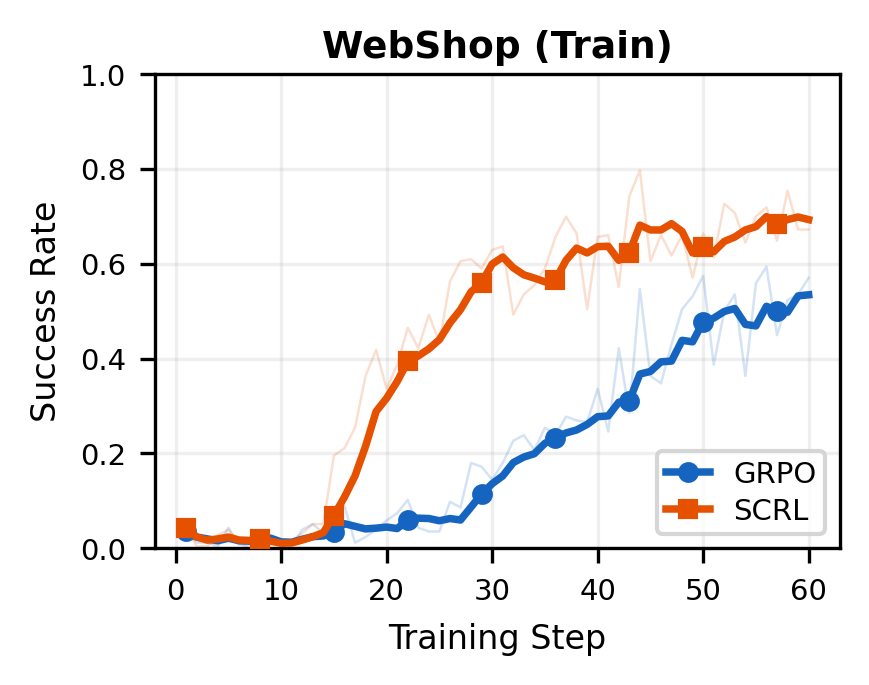
\includegraphics[width=0.32\textwidth]{figures/webshop_train_sr.png} &
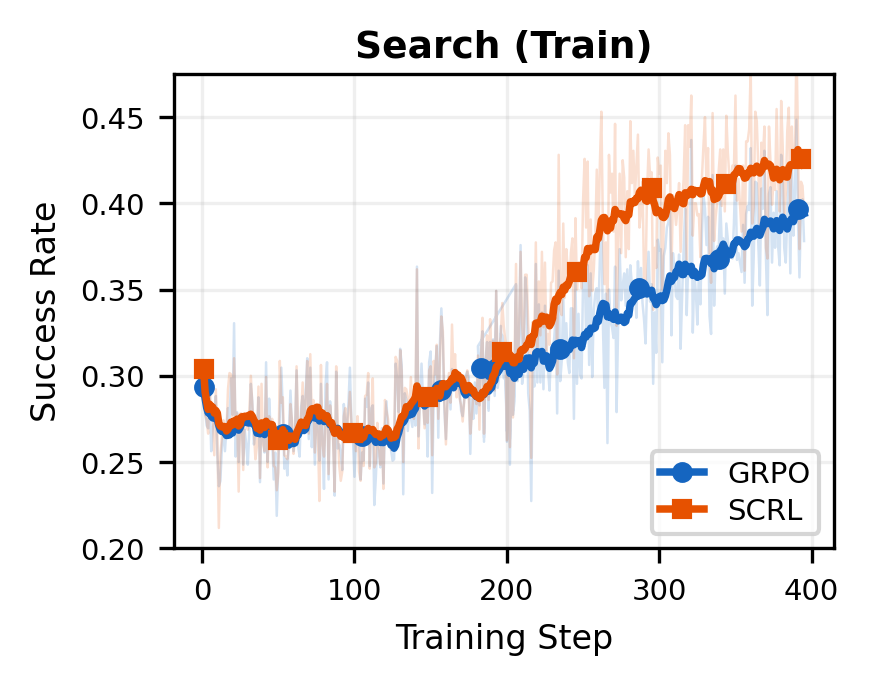
\includegraphics[width=0.32\textwidth]{figures/search_train_sr.png} &
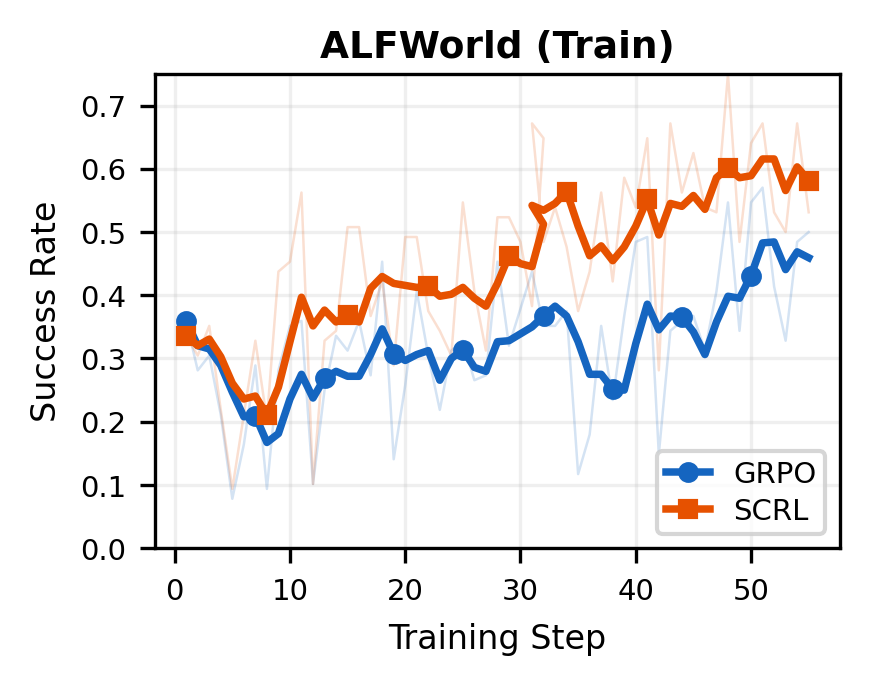
\includegraphics[width=0.32\textwidth]{figures/alfworld_train_sr.png} \\
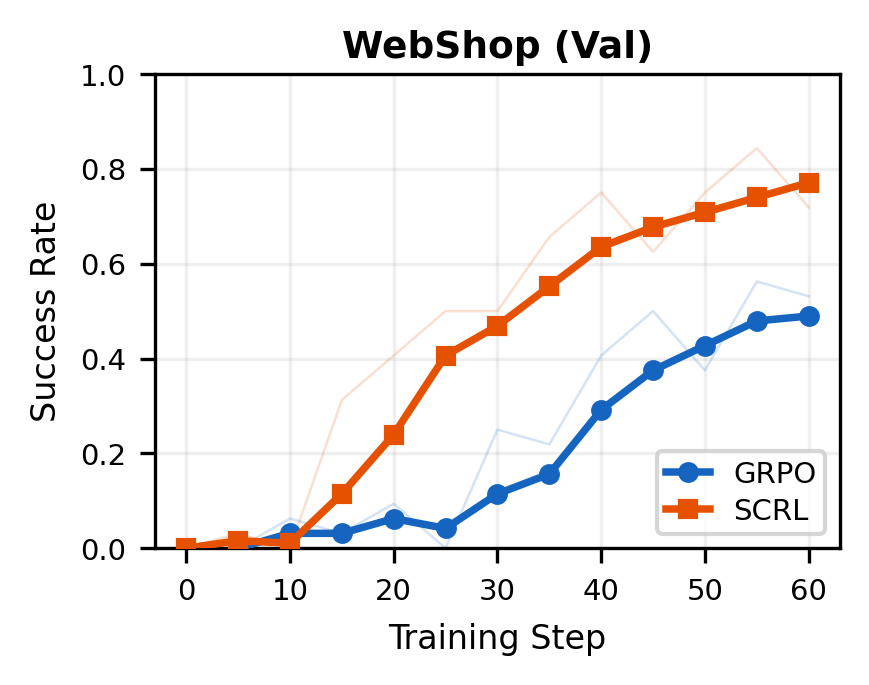
\includegraphics[width=0.32\textwidth]{figures/webshop_val_sr.png} &
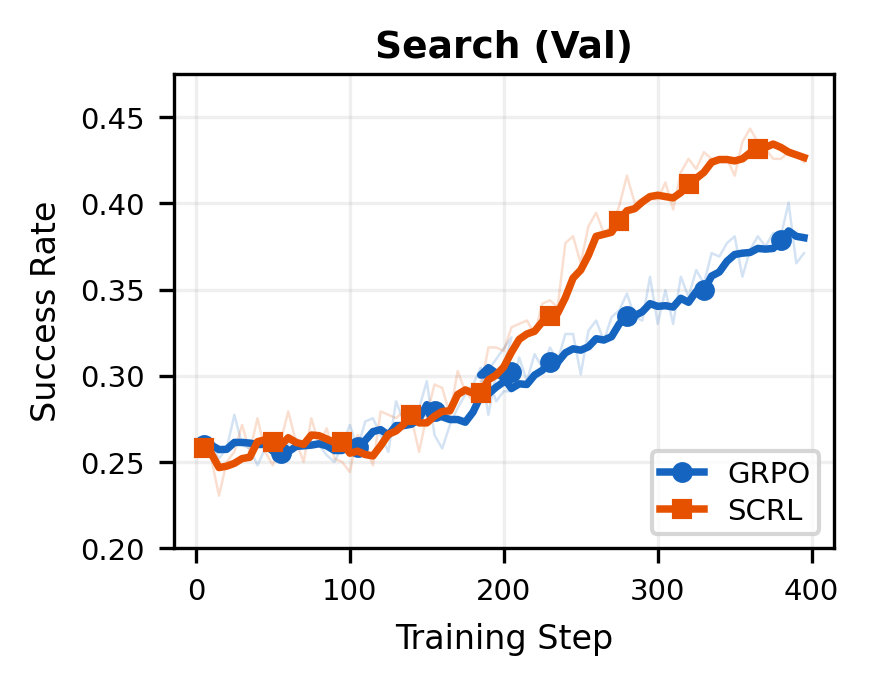
\includegraphics[width=0.32\textwidth]{figures/search_val_sr.png} &
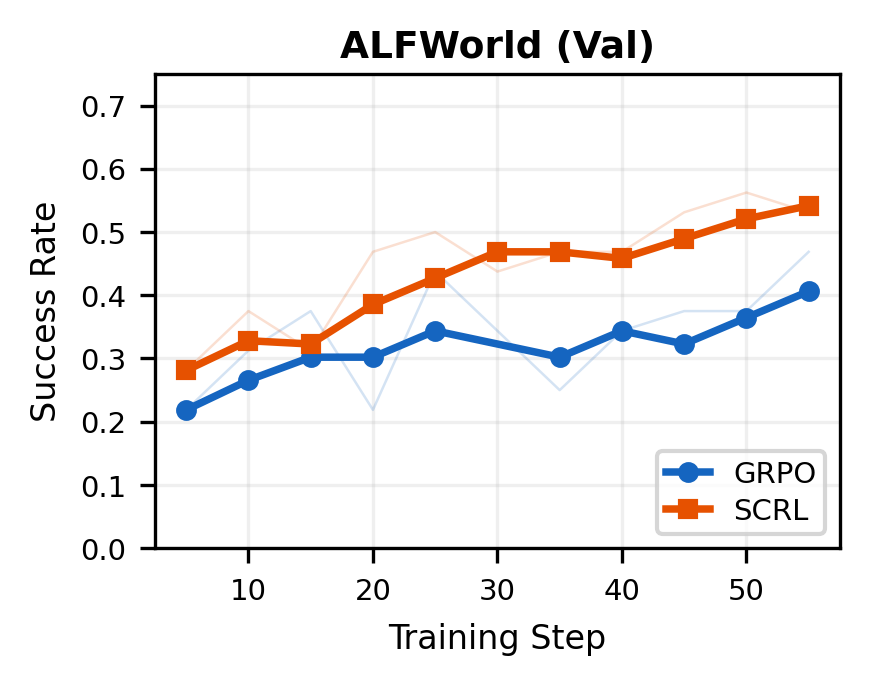
\includegraphics[width=0.32\textwidth]{figures/alfworld_val_sr.png}
\end{tabular}
\caption{Training (top) and validation (bottom) success rate on WebShop, Search, and ALFWorld. \ours~consistently converges faster than GRPO across all three benchmarks.}
\label{fig:results}
\end{figure*}

% TODO: Main results discussion

\subsection{Scaling Analysis}

\begin{figure*}[!t]
\centering
\begin{tabular}{@{}ccc@{}}
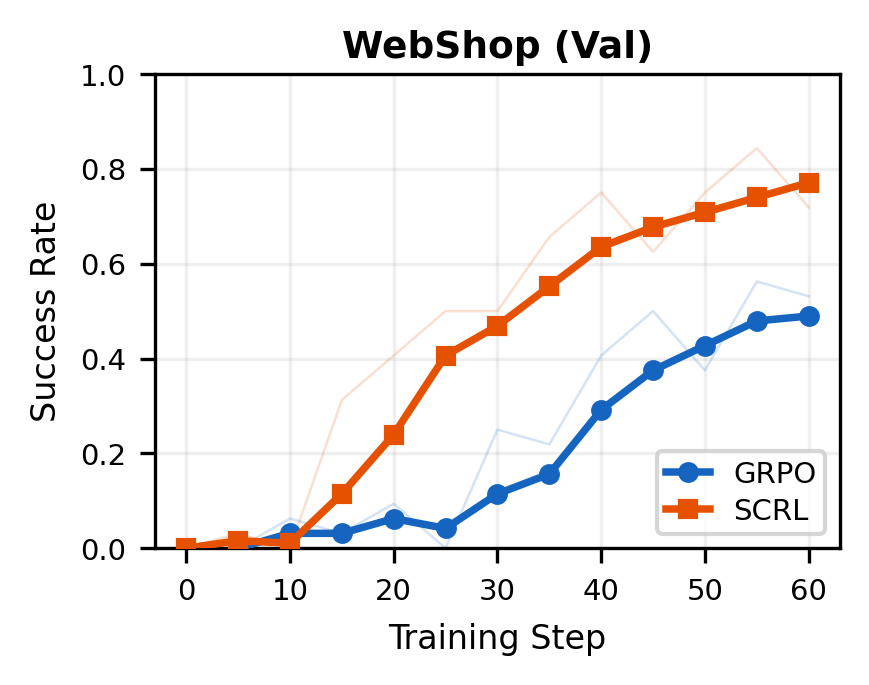
\includegraphics[width=0.32\textwidth]{figures/webshop_val_sr.png} &
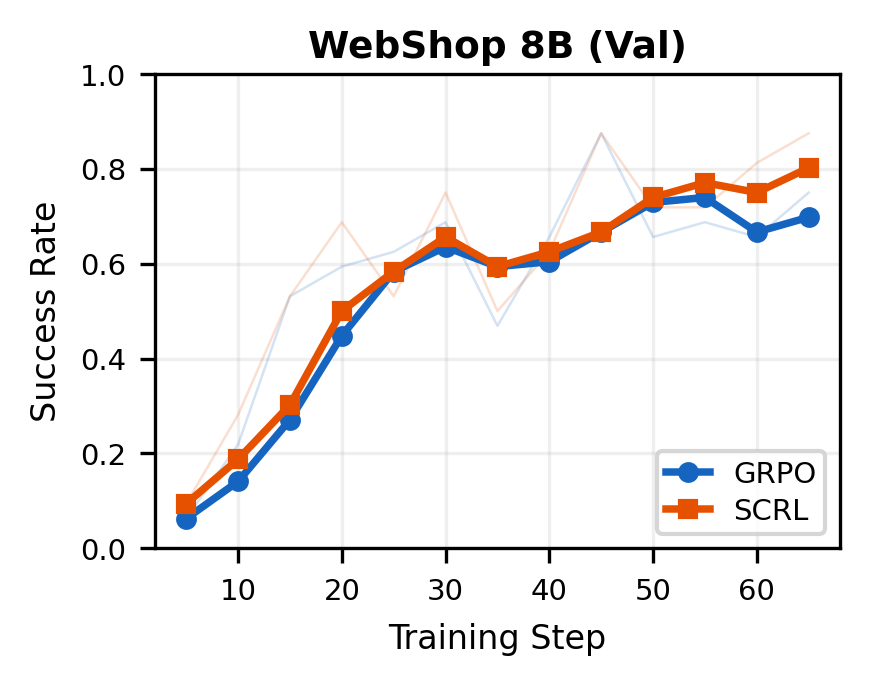
\includegraphics[width=0.32\textwidth]{figures/webshop_8b_val_sr.png} &
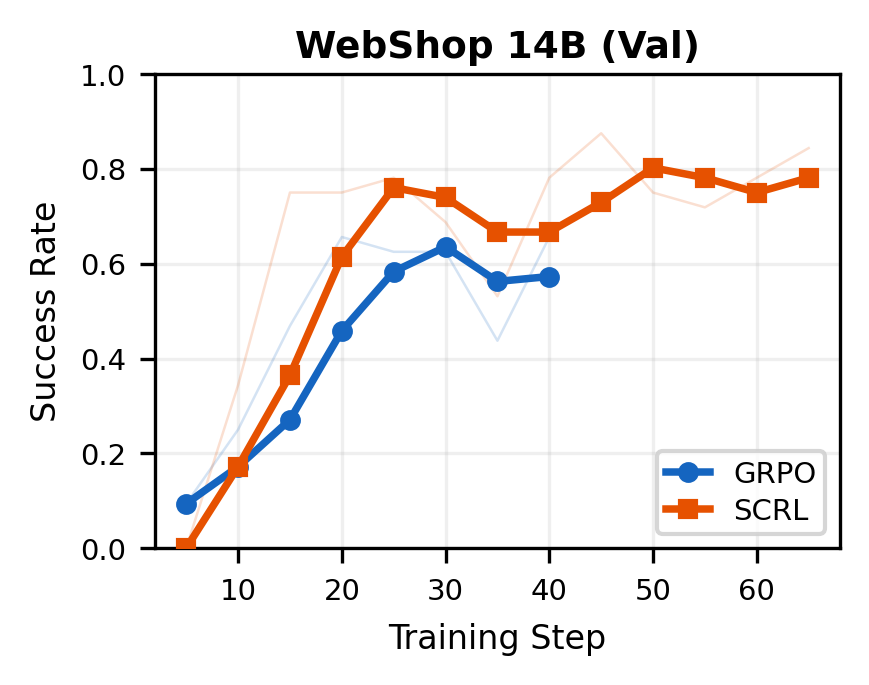
\includegraphics[width=0.32\textwidth]{figures/webshop_14b_val_sr.png}
\end{tabular}
\caption{WebShop validation success rate across model scales: 4B (left), 8B (middle), and 14B (right). \ours's advantage is largest at smaller scales and narrows as model capacity increases, consistent with the intuition that skills compensate most where model capacity is limited.}
\label{fig:scale}
\end{figure*}

% TODO: Scaling analysis discussion

\subsection{Ablation Studies}
\label{sec:ablation}

\begin{figure*}[!t]
\centering
\begin{tabular}{@{}ccc@{}}
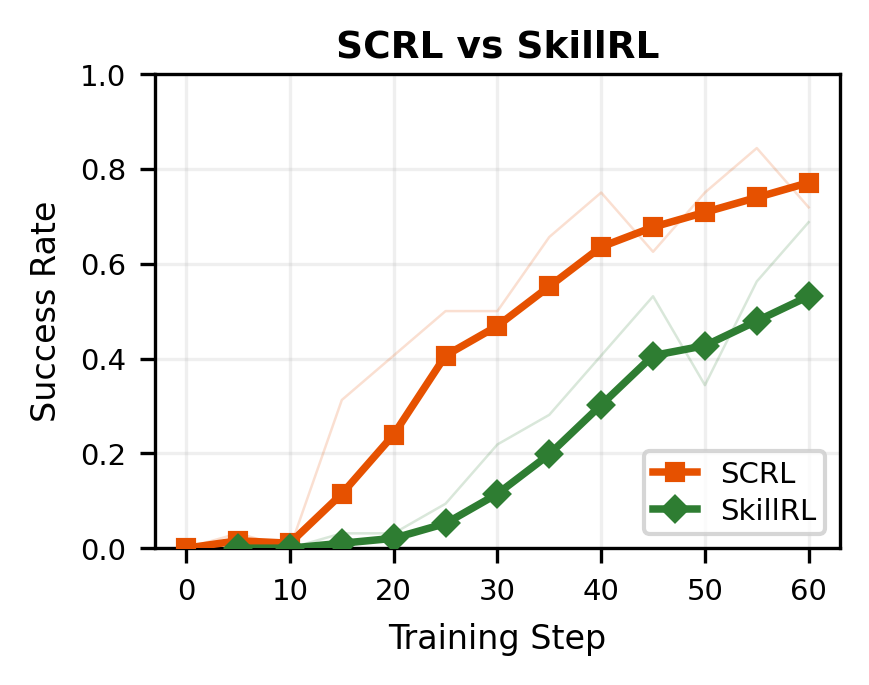
\includegraphics[width=0.32\textwidth]{figures/abl_skillrl_val_60.png} &
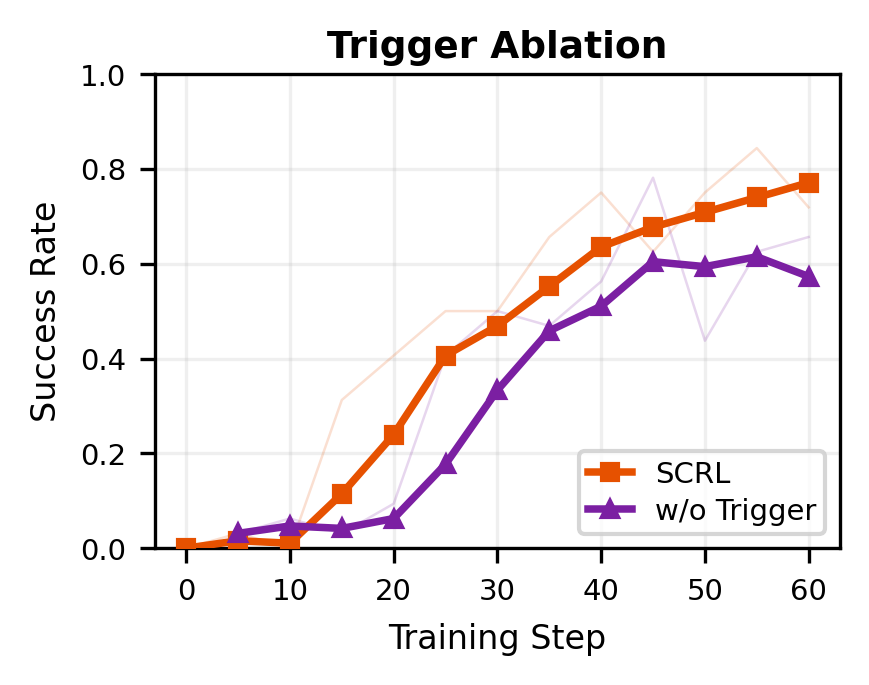
\includegraphics[width=0.32\textwidth]{figures/abl_trigger_val_60.png} &
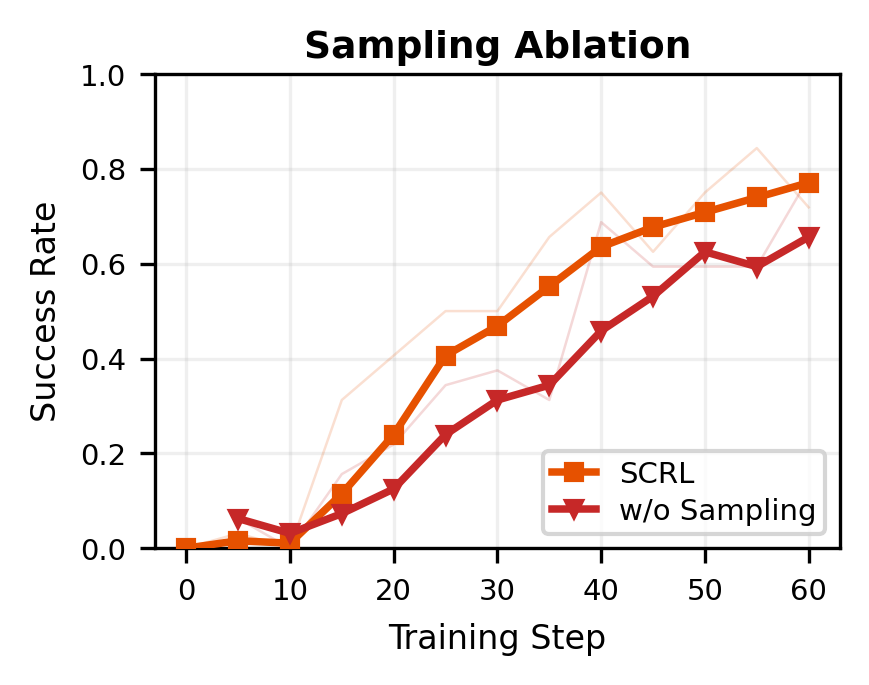
\includegraphics[width=0.32\textwidth]{figures/abl_sampling_val_60.png}
\end{tabular}
\caption{Ablation studies on WebShop validation success rate. Left: \ours~vs SkillRL (static skills). Middle: with vs without trigger conditions. Right: with vs without Thompson Sampling.}
\label{fig:ablation}
\end{figure*}

% TODO: Ablation analysis discussion


%=============================================================================
\section{Related Work}
\label{sec:related}
%=============================================================================

\sparagraph{Reinforcement Learning for LLMs}
Reinforcement learning has become a powerful paradigm for post-training LLMs, from alignment with human preferences \citep{ouyang2022training, rafailov2023direct} to reasoning via verifiable rewards. DeepSeek-R1 \citep{guo2025deepseek} demonstrated the effectiveness of RLVR, where GRPO \citep{shao2024deepseekmath} enables group-wise advantage estimation without a critic model. DAPO \citep{yu2025dapo} introduces training stability improvements such as clip-higher and dynamic sampling. Dr.~GRPO \citep{liu2025understanding} rectifies length bias. \ours~is orthogonal to these algorithmic improvements and can be integrated with any GRPO-based training pipeline.

\rparagraph{Tool-Integrated Agents}
LLM agents interact with environments through tool use \citep{yao2023react}. IRCoT \citep{trivedi-etal-2023-interleaving} interleaves chain-of-thought reasoning \citep{wei2022chain} with information retrieval. Toolformer \citep{schick2023toolformer} teaches tool usage via SFT. The RL paradigm has enabled multi-turn tool interactions \citep{feng2025retool, li2025torl}, with search tools excelling at question answering \citep{jin2025search, song2025r1}. End-to-end RL frameworks for tool use \citep{xue2025simpletir, jiang2025verltool} have grown rapidly, yet the role of \textit{dynamic skill guidance} during RL training has been largely unexplored: all existing approaches rely on static instructions designed before training begins.

\rparagraph{Skill and Instruction Optimization}
The performance of LLM agents is highly sensitive to their guiding instructions \citep{zhou2025multi}. Automated prompt optimization (APO) approaches use paraphrasing \citep{zhou2023large}, LLM-based optimizers \citep{yang2024large}, or textual gradients \citep{pryzant-etal-2023-automatic, 2025textgrad} to improve instructions, but operate offline. INSPO \citep{zhou2025inspo} is the first to integrate instruction optimization into the RL loop via a population-based approach with softmax-weighted sampling and successive halving \citep{jamieson2016non}. In the skill domain, Reflexion \citep{shinn2023reflexion} accumulates verbal feedback, ExpeL \citep{zhao2024expel} extracts experiential rules, MemRL \citep{zhang2026memrl} evolves episodic memory, and SkillRL \citep{xia2025skillrl} distills teacher-model skills for RL augmentation. Anthropic's Skill Creator \citep{anthropic2025skillcreator} pioneered the automated creation of modular, trigger-based skills from agent experience. \ours~builds on this paradigm but replaces the human judge with RL reward signals and integrates skill creation directly into the training loop, enabling online co-evolution rather than static augmentation.

\rparagraph{Bandit Methods for Online Selection}
Thompson Sampling \citep{thompson1933likelihood} is a Bayesian approach to the multi-armed bandit problem that maintains posterior distributions over arm rewards and samples actions proportionally to their probability of being optimal \citep{russo2018tutorial}. In the context of RL-based agent training, INSPO \citep{zhou2025inspo} uses softmax-weighted sampling over an instruction population. \ours~instead employs per-skill Thompson Sampling with trigger-gated counting: each skill maintains independent Beta posteriors updated only from episodes where its trigger fires, providing a natural handle for the heterogeneous activation patterns of different skill types.


%=============================================================================
\section{Conclusion}
\label{sec:conclusion}
%=============================================================================

We introduced \ours, a framework that enables the co-evolution of modular skills and policy learning for agentic RL. By integrating an assertion-driven skill creator pipeline with Thompson Sampling-based skill evolution directly into the GRPO training loop, \ours~achieves substantial convergence speedup with zero additional rollouts. The triple-duty design, where each GRPO rollout simultaneously provides policy gradients, failure data for skill creation, and bandit evaluation signals for skill evolution, demonstrates that significant efficiency gains are possible by extracting more value from existing training computation.

% TODO: Expand with specific results and future directions.


\bibliography{refs}
\bibliographystyle{plainnat}

\appendix

\section{Trigger Condition Types}
\label{app:triggers}

% TODO: Detail the specific trigger types (general, beginning, action\_pattern) with examples.

\end{document}
